\documentclass[12pt,a4paper]{article}

\usepackage[utf8]{inputenc}
\usepackage[T2A]{fontenc}
\usepackage[ukrainian]{babel}
\usepackage{geometry}
\geometry{
    left=2cm,
    right=2cm,
    top=2cm,
    bottom=2cm
}

\usepackage[table]{xcolor}
\usepackage{amsmath}
\usepackage{graphicx}
\usepackage{subcaption}
\usepackage{multirow}
\usepackage{makecell}
\usepackage{pdflscape}
\usepackage{array}
\newcolumntype{C}[1]{>{\centering\arraybackslash}m{#1}}

\usepackage[
  unicode,
  pdftitle={ІО-41, Давидчук А.М., АК. Частина 1, Лабораторна робота №2},
  pdfauthor={Давидчук Артем},
  pdfsubject={Архітектура Комп'ютерів. Частина 1}
]{hyperref}

\begin{document}

    \begin{titlepage}

        \begin{center}
\includegraphics[width=0.7\textwidth]{../../../TITLES/letterhead.png}\end{center}

        \begin{center}
            \large Національний технічний університет України\\
            «Київський політехнічний інститут імені Ігоря Сікорського»\\[1em]
            Факультет інформатики та обчислювальної техніки\\
            Кафедра обчислювальної техніки
        \end{center}

        \vfill

        \begin{center}
            \textbf{\LARGE Архітектура Комп'ютерів. Частина 1}\\[2em]
            \textbf{\Large Лабораторна робота №2}\\[0.5em]
            «Синтез блоків мікропрограмного управління» 
        \end{center}

        \vfill

        \begin{flushright}
            Виконав: студент 2 курсу ФІОТ, гр. ІО-41\\
            \textit{Давидчук А. М.}\\
            Залікова книжка № 4106\\[1em]
            Перевірив: \textit{Верба О.\,А.}
        \end{flushright}

        \vfill

        \begin{center}Київ --- 2026\end{center}

    \end{titlepage}

    \noindent
    \textbf{\underline{Тема:}} «Синтез блоків мікропрограмного управління».

    \vspace{1em}

    \noindent
    \textbf{\underline{Мета:}}  Дослідити засоби побудови блоків мікропрограмного управління.
    Одержати навички в проектуванні й налагодженні схем пристроїв управління
    з мікропрограмним управлінням.

    \begin{center} \textbf{\large Порядок виконання роботи} \end{center}

    \begin{enumerate}

        \item Варіанти завдання визначаються молодшими розрядами $a_7,\ldots,a_1$ двійкового номера залікової книжки.

        \item Розробити структурну схему операційного пристрою та змістовний мікроалгоритм обробки додатних чисел відповідно до завдання, наведеного у табл.~3.4 у методичних вказівках. Для побудови схеми використати комбінаційний суматор, регістр-лічильник циклів та асинхронні регістри, що мають входи управління зсувами і занесенням інформації. На структурній схемі повинні бути зазначені розрядність регістрів та шин.

        \item Розробити функціональну схему операційного пристрою.

        \item Виконати логічне моделювання роботи операційного пристрою за допомогою цифрової діаграми для вибраних значень операндів і їх розрядності.

        \item Побудувати структуру і функціональну схему БМУ, а також карту програмування ПМК для мікроалгоритму виконання заданої операції.

        \item Використовувати горизонтальне програмування зони управляючих сигналів. Врахувати дані, наведені у табл.~3.5 і 3.6 у методичних вказівках.

        \item Використовуючи моделюючу систему AFDK (ПРОГМОЛС~2.0) побудувати і налагодити пристрій для виконання заданої операції.

        \item На сконструйованому пристрої виконати числовий приклад і порівняти результат з одержаним при логічному моделюванні.

    \end{enumerate}

    \begin{center} \textbf{\large Хід роботи} \end{center}

    Мій номер залікової книжки: 4106, що у двіковому вигляді є 0001 0000 0000 1010.
    Звідси $a_7 = 0, a_6 = 0, a_5 = 0, a_4 = 1, a_3 = 0, a_2 = 1, a_1 = 0$.

    \vspace{1em}

    Звідси мій варіант завдання: \underline{Ділення, 2 способом}. Тобто обчислити функцію

    \[
    C = A \div B,
    \]

    Розрядність операндів -- 4 бітів;

    \vspace{1em}

    Спосіб адресації мікрокоманд: \underline{відносний};

    \vspace{1em}

    Ємність ПМК -- 16 бітів;

    \vspace{1em}

    Область $\beta_4$ –- перевірка на парність (де непарний = 1).

    \vspace{1em}

    Тривалість МО підсумовування: 4 тактів (всі інші операції мають тривалість в один такт).

    \newpage

    \noindent
    Операційна схема пристрою для виконання операції ділення другим способом для 4-розрядних операндів:

    \begin{figure}[h!]
        \centering
        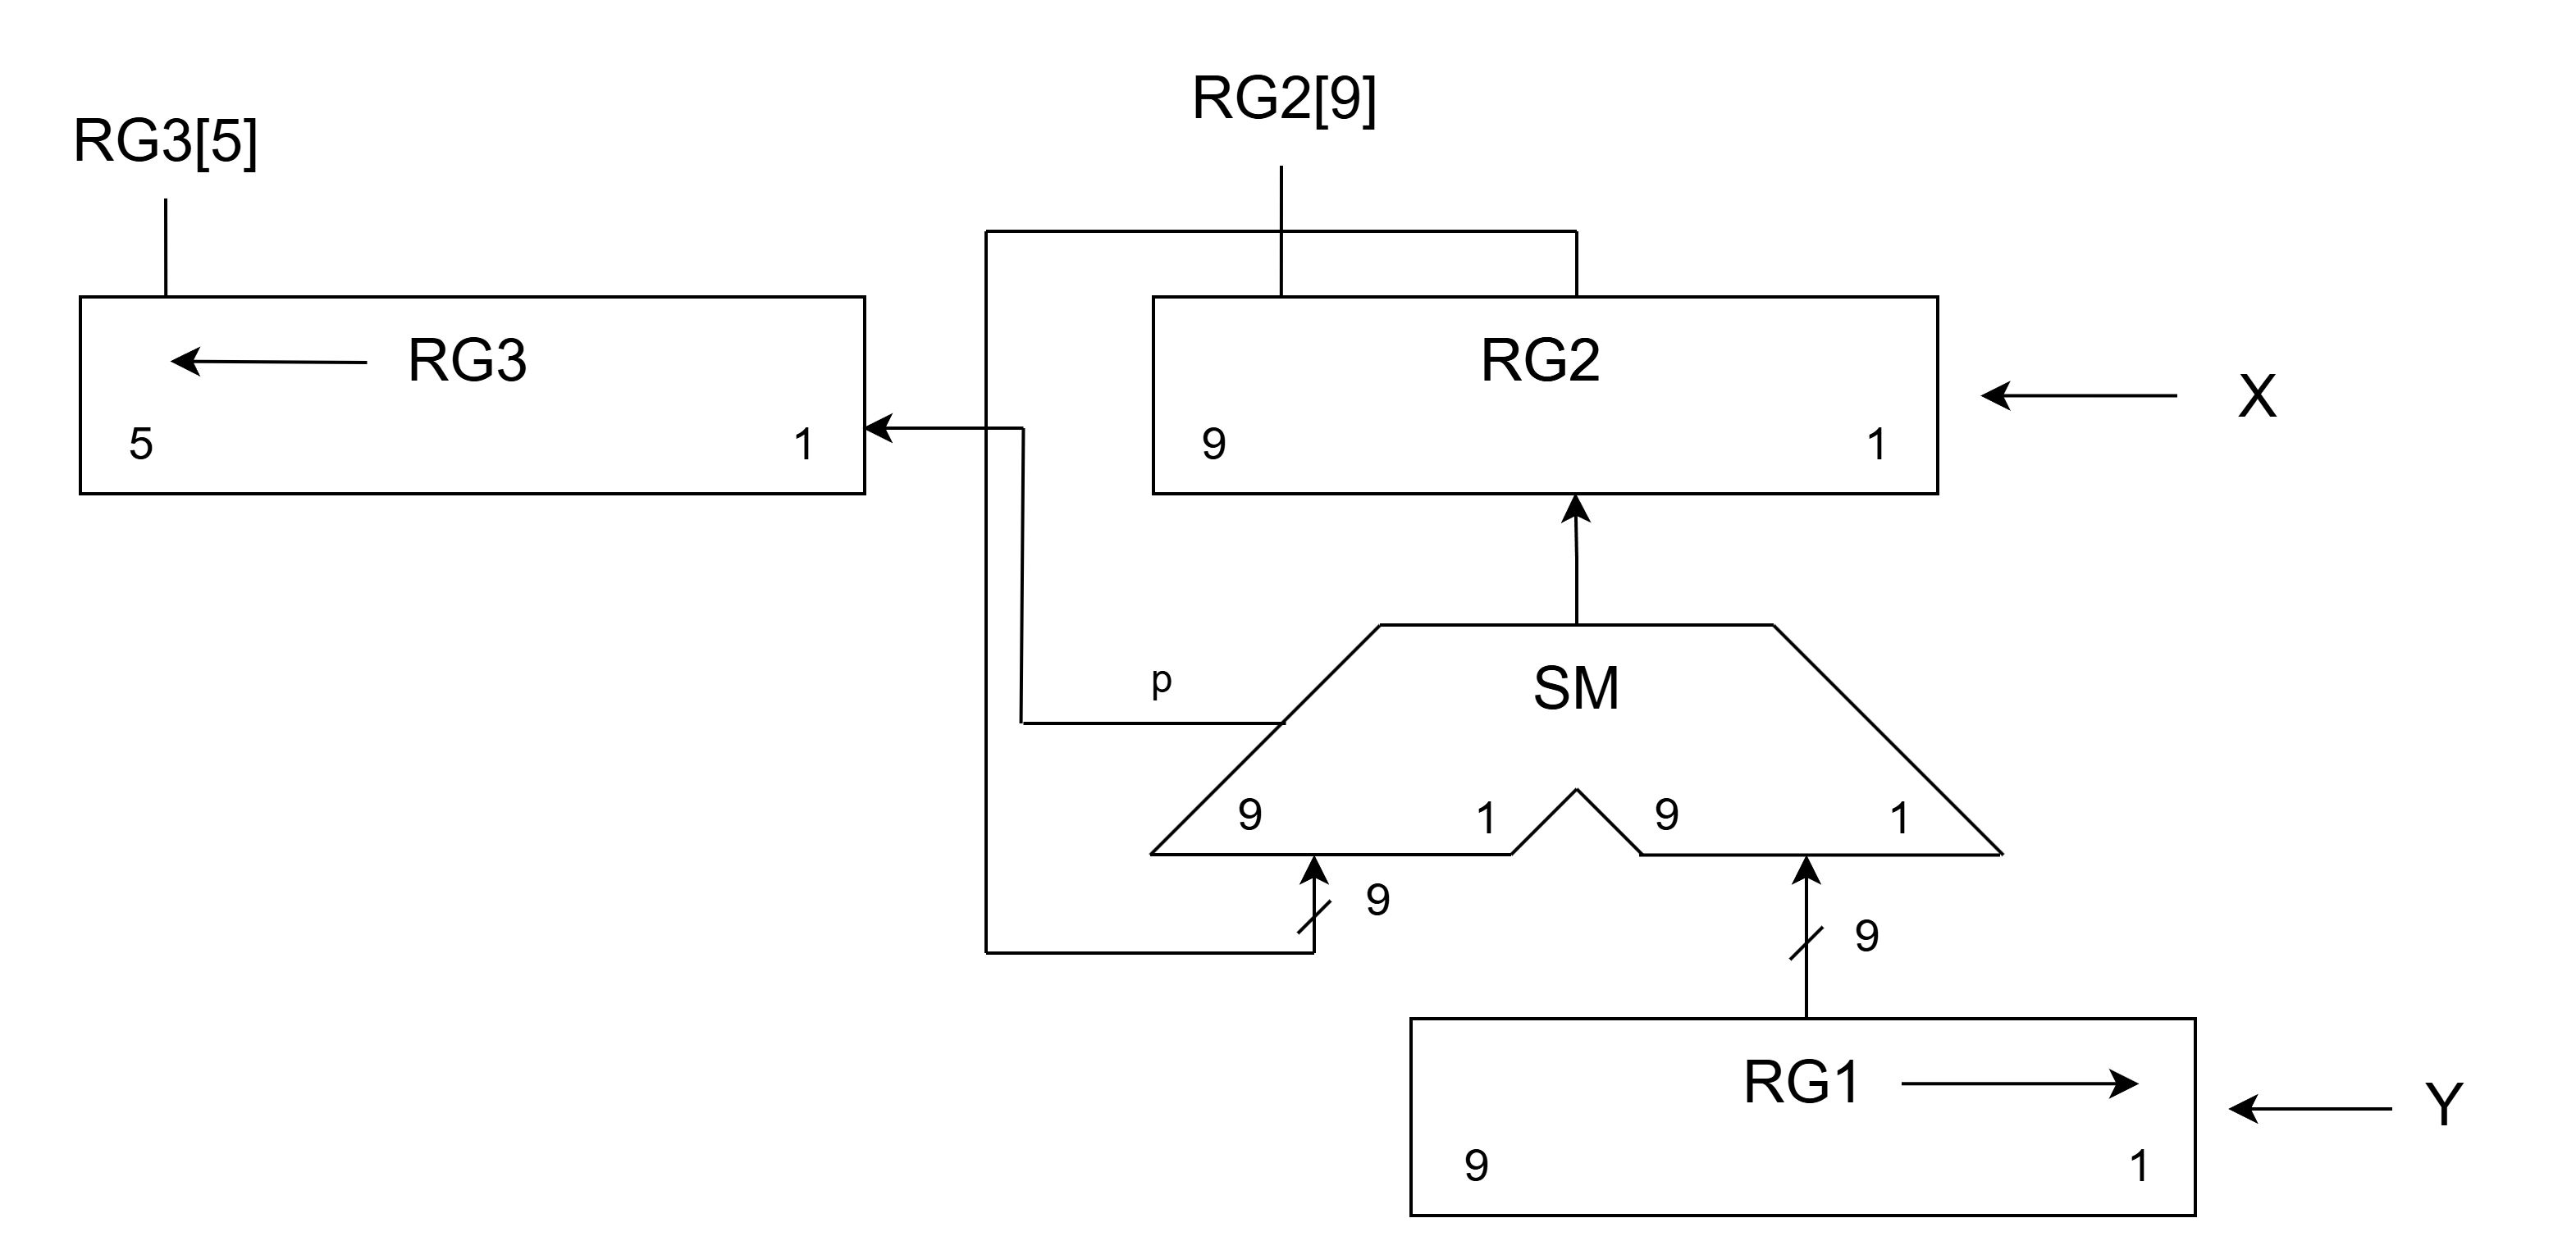
\includegraphics[width=0.8\linewidth]{media/op4.png}
        \caption{Операційна схема ділення 2 способом для 4 розрядних операндів}
    \end{figure}

    \noindent
    Функціональна схема пристрою для виконання операції ділення другим способом для 4-розрядних операндів:

    \begin{figure}[h!]
        \centering
        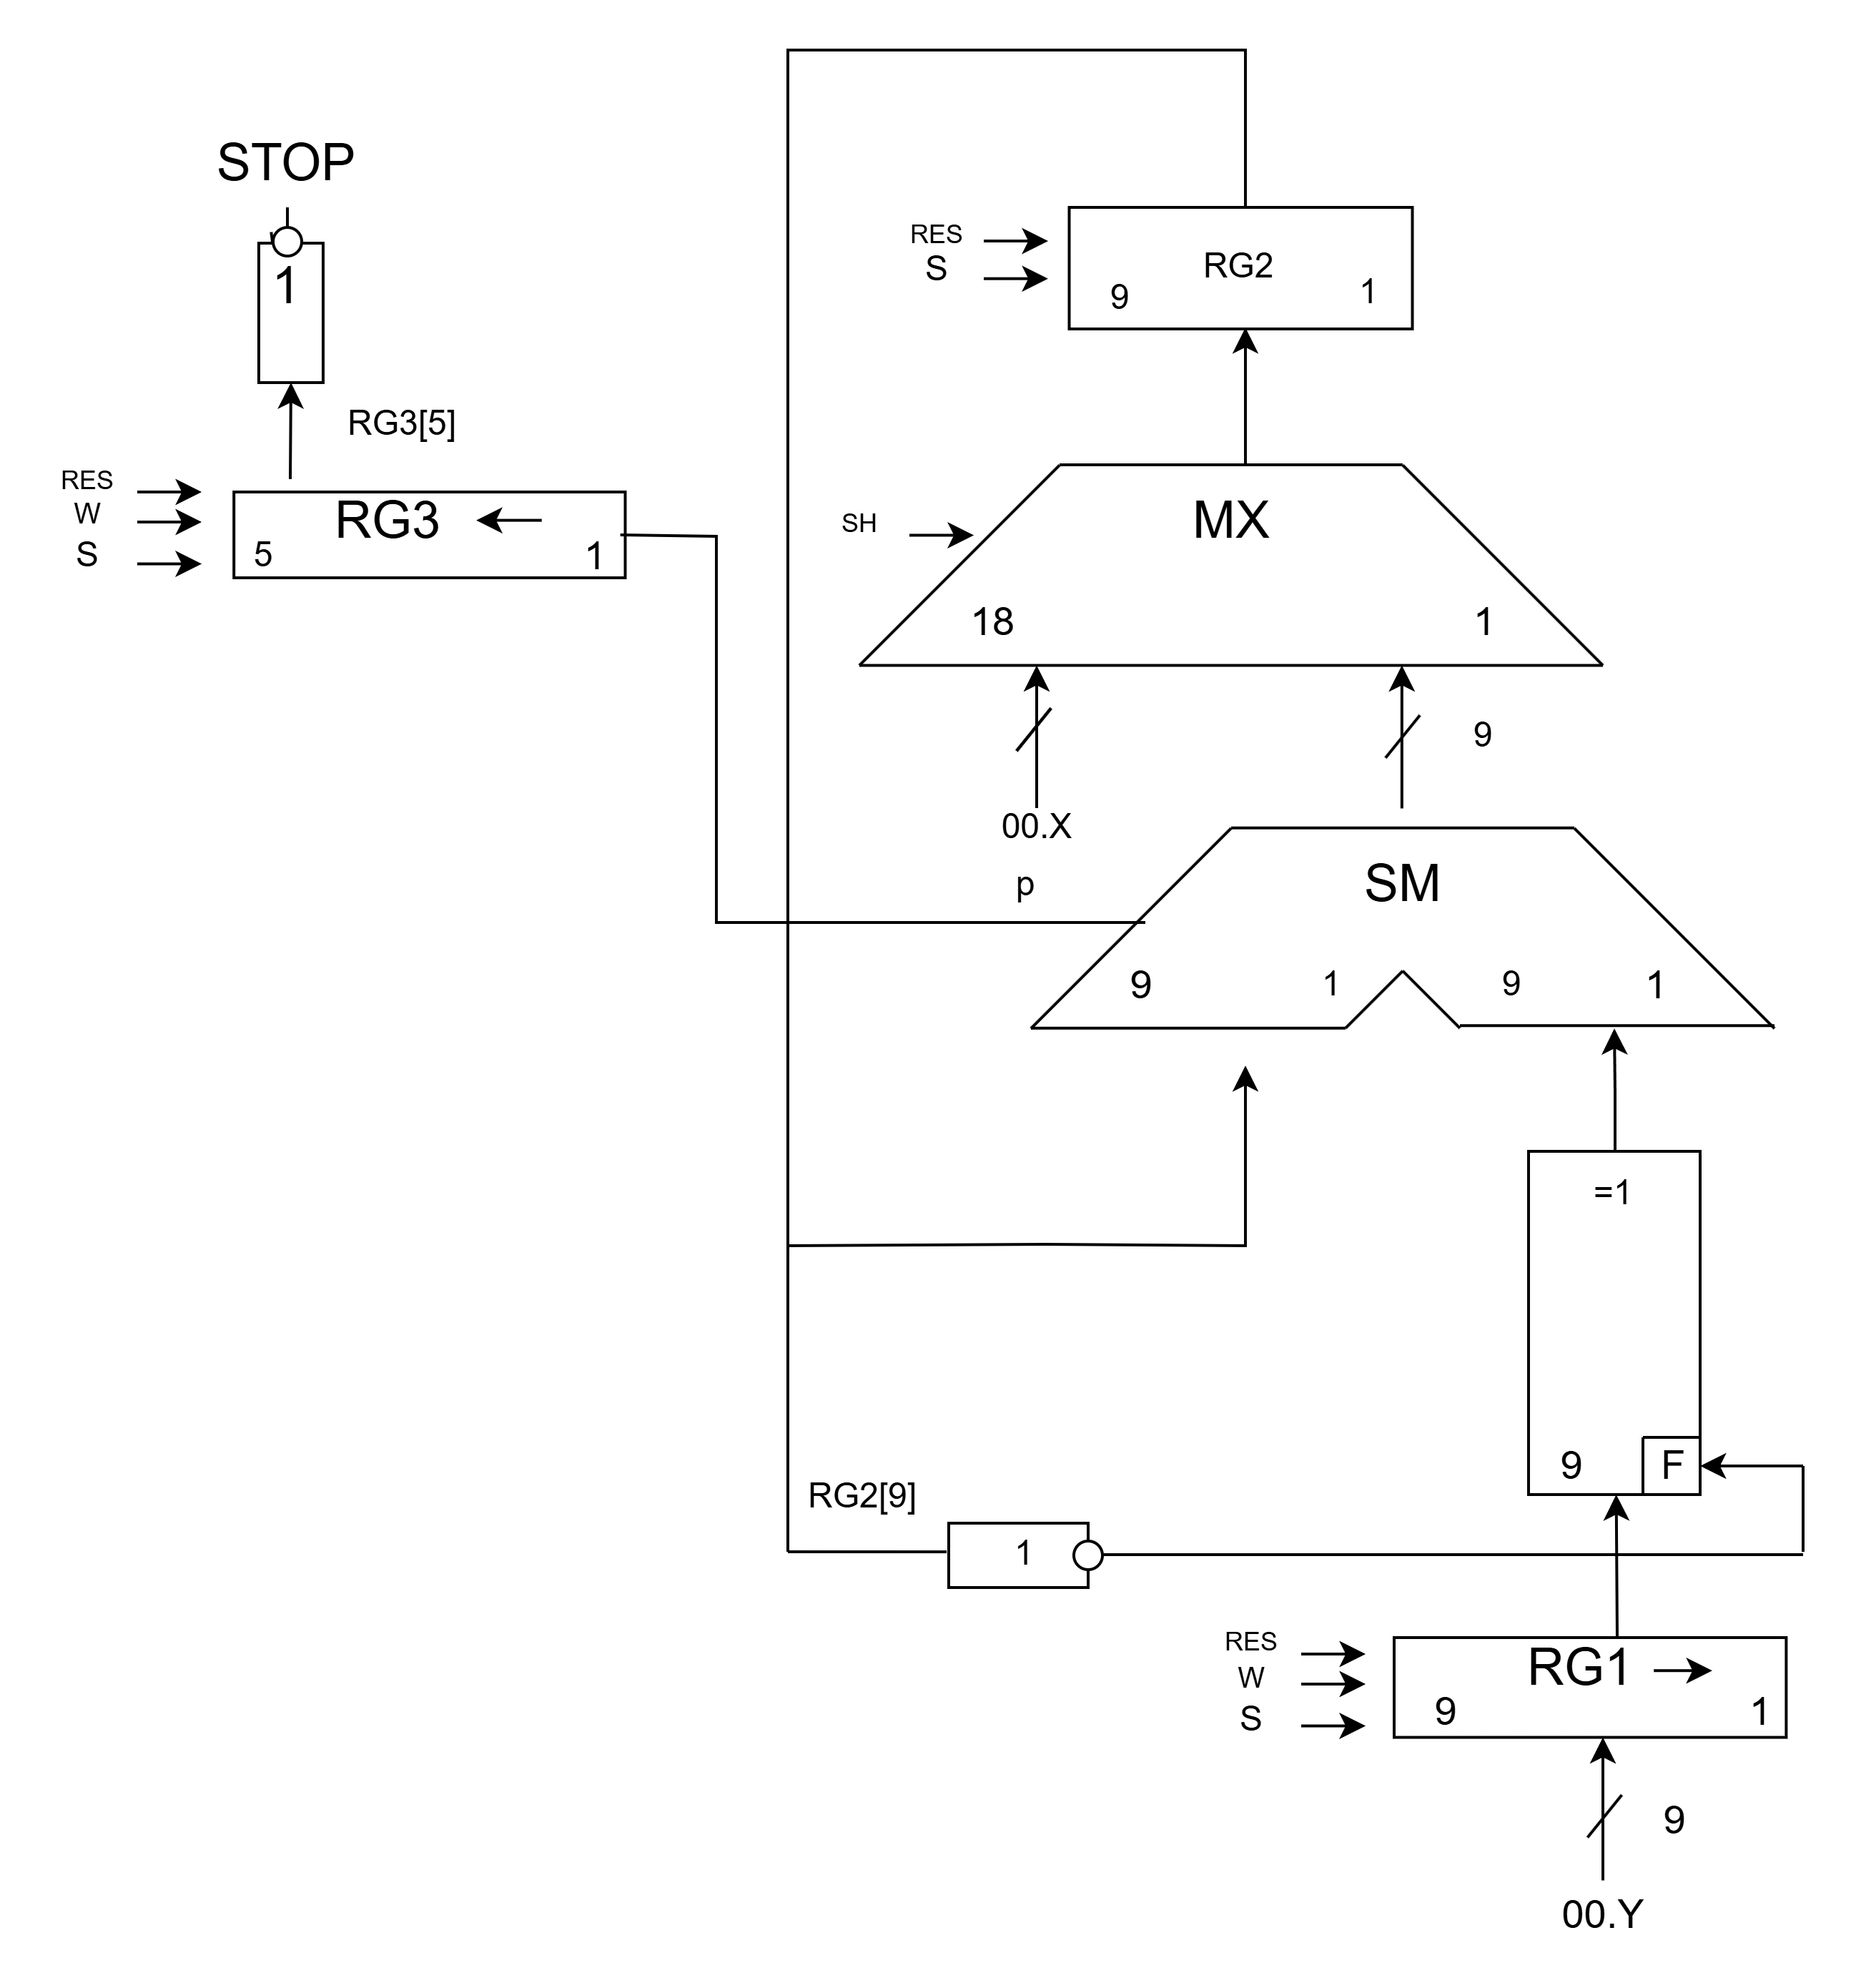
\includegraphics[width=0.7\linewidth]{media/func4.png}
        \caption{Функціональна схема ділення 2 способом для 4 розрядних операндів}
    \end{figure}

    \newpage

    \noindent
    Структурний мікроалгоритм виконання 2 способу ділення для 4 розрядних операндів:

    \begin{figure}[h!]
        \centering
        
\includegraphics[width=0.7\linewidth]{media/str_alg.png}
        \caption{Стуктурний мікроалгоритм ділення 2 способом для 4 розрядних операндів}
    \end{figure}

    \newpage

    \noindent
    Функціональний мікроалгоритм виконання 2 способу ділення для 4 розрядних операндів:

    \begin{figure}[h!]
        \centering
        
\includegraphics[width=0.5\linewidth]{media/func_alg.png}
        \caption{Функціональний мікроалгоритм ділення 2 способом для 4 розрядних операндів}
    \end{figure}

    \newpage

    \noindent
    Закодований мікроалгоритм виконання 2 способу ділення для 4 розрядних операндів:

    \begin{figure}[h!]
        \centering
        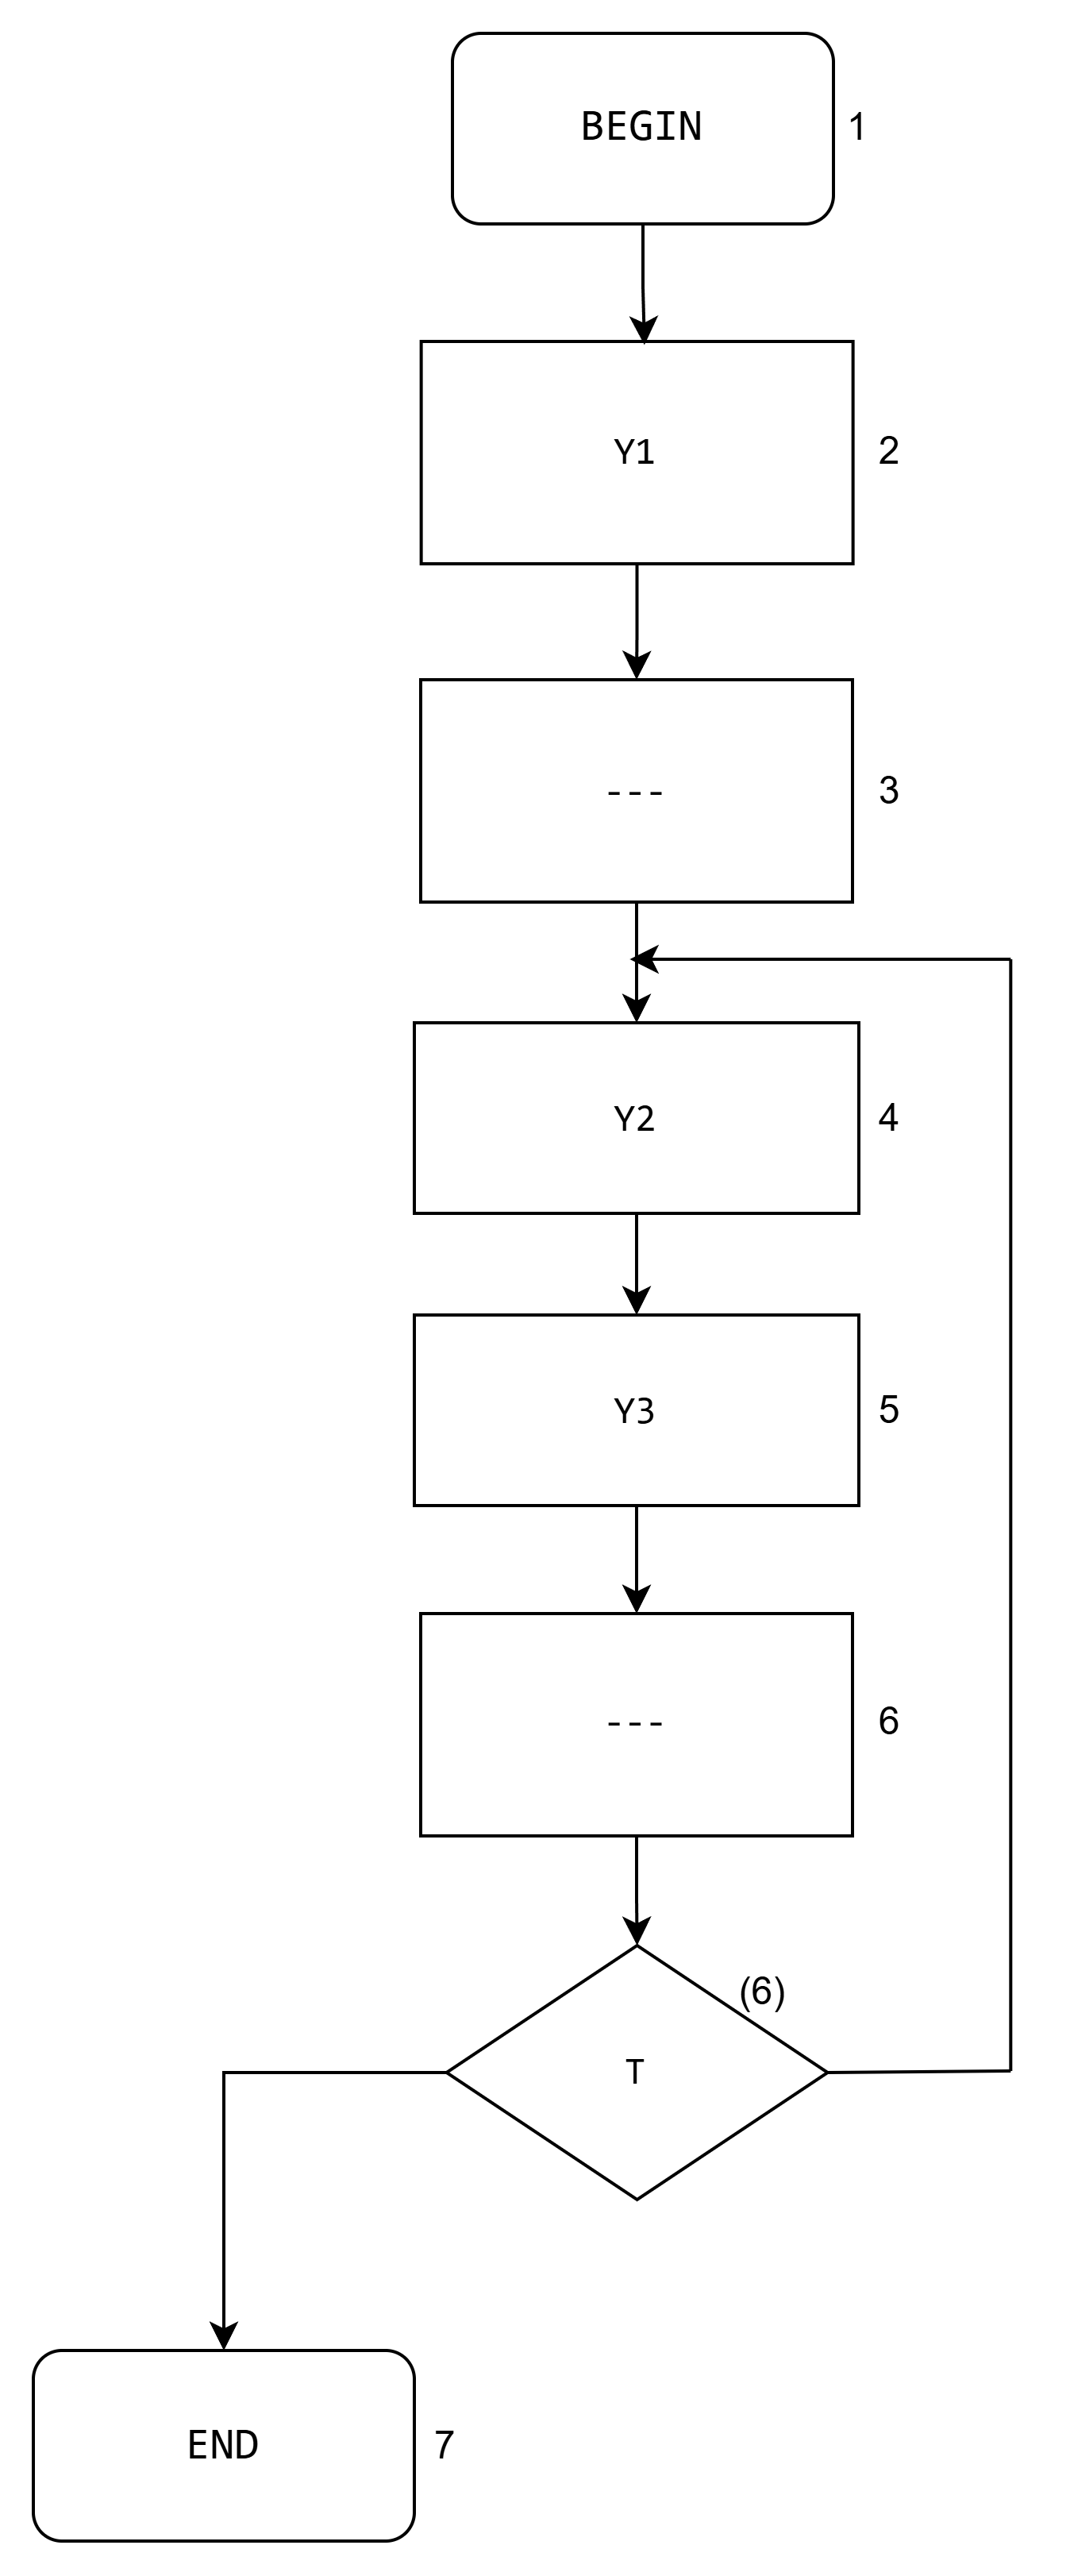
\includegraphics[width=0.5\linewidth]{media/code_alg.png}
        \caption{Закодований мікроалгоритм ділення 2 способом для 4 розрядних операндів}
    \end{figure}

    \newpage

    \noindent
    Проведемо ділення для чисел $X = 0010$, $Y = 0100$,:

    \begin{table}[h!]
        \centering
        \renewcommand{\arraystretch}{1.3}
        \begin{tabular}{|c|c|c|c|p{6.5cm}|}
            \hline
            \textbf{№} &
            \makecell{\textbf{RG3} \\[0.3em] 5 - 1} &
            \makecell{\textbf{RG2} \\[0.3em] 9 - 1} &
            \makecell{\textbf{RG1} \\[0.3em] 9 - 1} &
            \textbf{Мікрооперації} \\
            \hline
            \textbf{0} &
            \makecell[l]{11111} &
            \makecell[l]{001000000} &
            \makecell[l]{010000000 \\ 110000000} &
            \makecell[l]{
                \texttt{RG3 := 1..11;} \\
                \texttt{RG2 := X.0..0;} \\
                \texttt{RG1 := Y.0..0;}
            } \\
            \hline

            \textbf{1} &
            \makecell[l]{<<11110} &
            \makecell[l]{
                001000000 \\
                +110000000 \\
                =0|111000000
            } &
            \makecell[l]{
                >>001000000 \\
                >>111000000
            } &
            \makecell[l]{
                \texttt{RG2 := RG2 + RG1;} \\
                \texttt{RG3 := L(RG3).SM[P]} \\
                \texttt{RG1 := 0.R(RG1)}
            } \\
            \hline

            \textbf{2} &
            \makecell[l]{<<11101} &
            \makecell[l]{
                111000000 \\
                +001000000 \\
                =1|000000000
            } &
            \makecell[l]{
                >>000100000 \\
                >>111100000
            } &
            \makecell[l]{
                \texttt{RG2 := RG2 + !RG1 + D;} \\
                \texttt{RG3 := L(RG3).SM[P]} \\
                \texttt{RG1 := 0.R(RG1)}
            } \\
            \hline

            \textbf{3} &
            \makecell[l]{<<11010} &
            \makecell[l]{
                000000000 \\
                +111100000 \\
                =0|111100000
            } &
            \makecell[l]{
                >>000010000 \\
                >>111110000
            } &
            \makecell[l]{
                \texttt{RG2 := RG2 + RG1;} \\
                \texttt{RG3 := L(RG3).SM[P]} \\
                \texttt{RG1 := 0.R(RG1)}
            } \\
            \hline

            \textbf{4} &
            \makecell[l]{<<10100} &
            \makecell[l]{
                111100000 \\
                +000010000 \\
                =0|111110000
            } &
            \makecell[l]{
                >>000001000 \\
                >>111111000
            } &
            \makecell[l]{
                \texttt{RG2 := RG2 + !RG1 + D;} \\
                \texttt{RG3 := L(RG3).SM[P]} \\
                \texttt{RG1 := 0.R(RG1)}
            } \\
            \hline

            \textbf{5} &
            \makecell[l]{<<01000} &
            \makecell[l]{
                111110000 \\
                +000001000 \\
                =0|111111000
            } &
            \makecell[l]{
                >>000000100 \\
                >>111111100
            } &
            \makecell[l]{
                \texttt{RG2 := RG2 + !RG1 + D;} \\
                \texttt{RG3 := L(RG3).SM[P]} \\
                \texttt{RG1 := 0.R(RG1)}
            } \\
            \hline
        \end{tabular}
    \end{table}

    \noindent
    Тобто $C = X / Y \approx 1000$

    \vspace{1em}

    \noindent
    Тепер визначимо розряднів частино слова МК, тобто для $\beta_1$, $\beta_2$, $\beta_3$ та $\beta_4$.

    Так як у нас спосіб адресації відносний, то $\beta_1$ матиме такі частини $S$ та $M$, звідси

    \[
    n_{\beta_1} = n_S + n_M
    \]

    де $S$ -- максимальне можливе число приросту. Так як у нас слово ПМК містить 16 комірок, це означає що для представлення всіх команд досить мати адреси в довжину 4 біти, бо $2^4 = 16$, тобто якщо адреса має 4 розряди, то вона здатна посилатись на 16 різних мікрокоманд. Звідси максимальний приріст $N = 4$, і тепер ми можемо визначити розмір $n_S$:

    \[
    n_S = ]\log_2(N)[ + 1 = ]\log_2(4)[ + 1 = 2 + 1 = 3
    \]

    А розрядність $n_M$ можемо знайти за такою формулою:

    \[
    n_M = ] \log_2(k+2) [
    \]

    де $k$ -- кількість вхідних, умов, що в нашому випадку $k=1$. Звідси

    \[
    n_M = ] \log_2(1+2) [ = ] \log_2(3) [ = 2
    \]

    Тобто $n_{\beta_1} = n_S = n_M = 2 + 3 = 5$ бітів. Тепер розряхуємо для $\beta_2$. Так як у нас кодування $\beta_2$ є горизонтальним, звідси розрядність цієї ділянки дорівнює кількості вихідних керуючих сигналів, що в нашому випадку 3. Тобто $n_{\beta_2} = 3$.

    Для розряхунку $\beta_3$, ми використаємо таку формулу:

    \[
    n_{\beta_3} =]\log_2(r)[+1
    \]

    де $r$ -- максимальна часова затримка мікрооперації. Так як у цій лабораторній роботі тривалість операції всіх операцій окрім сумування дорівнюють 1, то максимальна тривалість операції дорівнює тривалості сумування. Звідси і максимальна затримка мікрооперацій дорівнює затримці операції підсумовування. Для обчислення затримки операції підсумовування, потрібно відняти один такт із кількості тактів тривалості, тобто
    
    \[
    \Delta t = t - 1
    \]

    де $t$ -- тривалість операції підсумовування, а $\Delta t$ -- його затримка. Так як у нас $t = 4$, звідси $\Delta t = 4 - 1 = 3$ такта, тобто $r = \Delta t$. Звідси
    
    \[
    n_{\beta_3} =] \log_2(3)[ +1 = 2+1 = 3 
    \]

    Тепер порахуємо розрядність для $\beta_4$. Так як у нас вона буде слугувати лише для перевірки на парність, це означає, що для $\beta_4$ вистачить один біт, тобто $n_{\beta_4} = 1$.

    Звідси перевіримо, чи сума розрядів частин слова МК $\beta_1$, $\beta_2$, $\beta_3$ та $\beta_4$ не перевищує 16:

    \[
    n_{\beta_1} + n_{\beta_2} + n_{\beta_3} + n_{\beta_4} = 5 + 3 + 3 + 1 = 12 < 16
    \]

    \noindent
    Побудуємо таблицю формування сигналів мультиплексора:

    \begin{table}[h]
    \centering
    \begin{tabular}{|c|c|c|}
        \hline
        $M_2$ & $M_1$ & OUT\\
        \hline
        0 & 0 & 0 \\
        \hline
        0 & 1 & - \\
        \hline
        1 & 0 & X \\
        \hline
        1 & 1 & 1 \\
        \hline
    \end{tabular}
    \caption{Таблиця кодування вихідних сигналів мультиплексора}
    \end{table}

    \noindent
    А тепер побудуємо схематичне зображення мікрокоманд, та переходи між ними:

    \begin{figure}[h!]
        \centering
        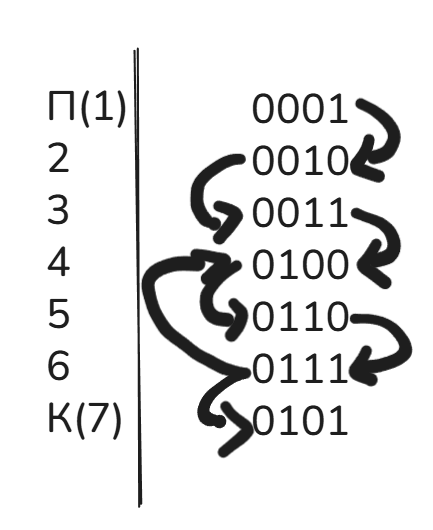
\includegraphics[width=0.4\linewidth]{media/mom.png}
        \caption{Cхематичне зображення мікрокоманд та їх переходів}
    \end{figure}

    Щоб представити затримку в $\beta_3$, ми маємо $-3$ представити в ДК коді, що буде дорівнювати: $-3 = 1.11 = 1.00 + 0.01  = 1.01$

    \newpage

    Тепер на основі всіх попередніх досліджень побудуємо карту програмування БМУ:

    \begin{table}[h!]
        \centering
        \renewcommand{\arraystretch}{1.3}
        \begin{tabular}{|c|c|cc|ccc|cc|c|}
            \hline
            \multirow{2}{*}{№ мк} & \multirow{2}{*}{Адреса} & \multicolumn{2}{c|}{$\beta_1$} & \multicolumn{3}{c|}{$\beta_2$} & \multicolumn{2}{c|}{$\beta_3$} & \multirow{2}{*}{$\beta_4$} \\
            \cline{3-9}
            &  & $S$ & $M$ & $y_1$ & $y_2$ & $y_3$ & ЗН & $\Delta$ &  \\
            \hline
            П(1) & 0001 & 001 & 00 & 0 & 0 & 0 & 0 & 00 & 1 \\
            \hline
            2    & 0010 & 001 & 00 & 1 & 0 & 0 & 0 & 00 & 0 \\
            \hline
            3    & 0011 & 001 & 00 & 0 & 0 & 0 & 0 & 00 & 1 \\
            \hline
            4    & 0100 & 010 & 00 & 0 & 1 & 0 & 1 & 01 & 0 \\
            \hline
            5    & 0110 & 001 & 00 & 0 & 0 & 1 & 0 & 00 & 0 \\
            \hline
            6    & 0111 & 101 & 10 & 0 & 0 & 0 & 0 & 00 & 1 \\
            \hline
            К(7) & 0101 & 000 & 00 & 0 & 0 & 0 & 0 & 00 & 0 \\
            \hline
        \end{tabular}
    \end{table}

    \noindent
    Тепер побудуємо схему в AFDK, та проведемо обчислення:

    \begin{figure}[h!]
        \centering
        
\includegraphics[width=\linewidth]{media/scheme.png}
        \caption{Схема в AFDK}
    \end{figure}

    \newpage

    \noindent
    Часова діаграма роботи БМУ:

    \begin{figure}[h!]
        \centering
        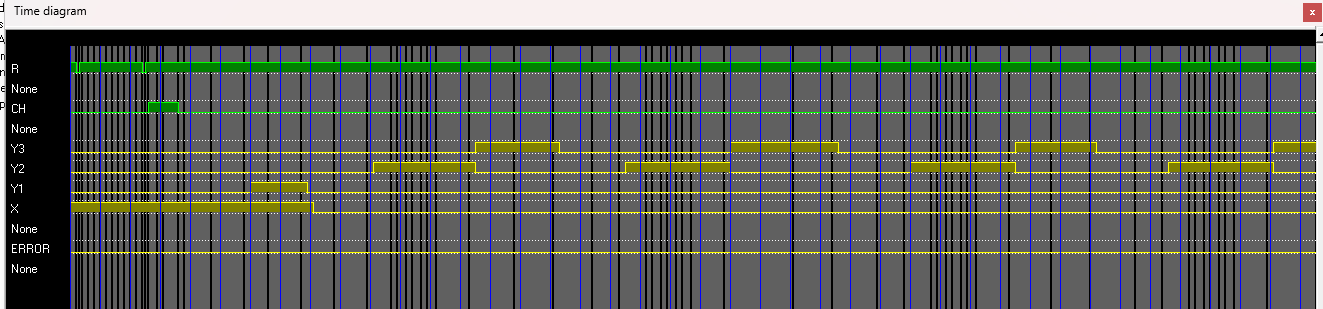
\includegraphics[width=\linewidth]{media/tim0.png}
        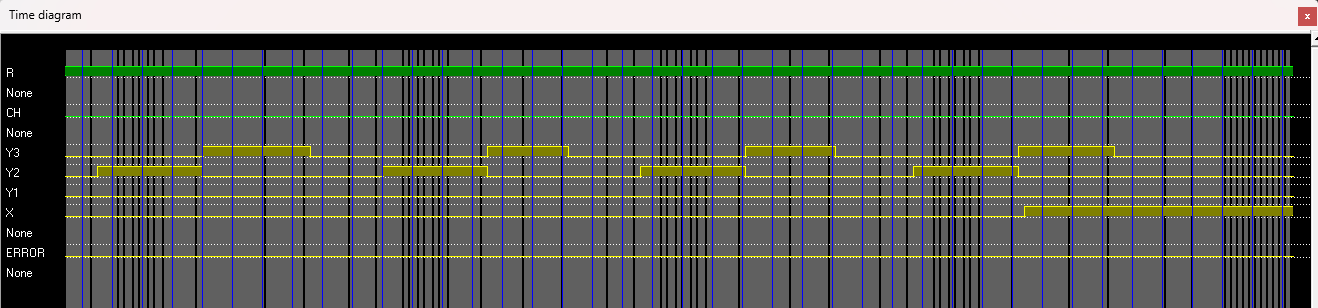
\includegraphics[width=\linewidth]{media/tim1.png}
        \caption{Часові діаграми}
    \end{figure}

    Результат ділення -- 1000, що співпадає із ручно обчисленим значенням зі таблиці станів реістрів, що свідчить про коректну роботу АЛП із БМУ.

    \begin{center} \textbf{\large Висновок}\end{center}

    У ході виконання лабораторної роботи було досліджено принципи побудови блоків мікропрограмного управління та отримано практичні навички проектування пристроїв керування з мікропрограмним управлінням. Для заданого варіанта було розроблено операційну та функціональну схеми пристрою, що реалізує операцію ділення другим способом для 4-розрядних додатних чисел.

    У процесі роботи було побудовано структурний, функціональний і закодований мікроалгоритми виконання операції, визначено структуру слова мікрокоманди, обчислено розрядності полів $\beta_1$, $\beta_2$, $\beta_3$ та $\beta_4$, а також перевірено відповідність сумарної розрядності заданій ємності ПМК. На основі отриманих результатів було сформовано карту програмування постійної мікропрограмної пам’яті та побудовано функціональну схему блоку мікропрограмного управління.

    За допомогою моделюючої системи AFDK було реалізовано та налагоджено розроблений пристрій, а також виконано перевірку його роботи на числовому прикладі. Аналіз часових діаграм підтвердив правильність формування керуючих сигналів блоком мікропрограмного управління та коректність виконання операції ділення. Отримані результати логічного моделювання збігаються з результатами, одержаними в моделюючій системі, що підтверджує працездатність і правильність спроектованого пристрою.

    \begin{center} \textbf{\large Відповіді на контрольні запитання} \end{center}

    \begin{enumerate}
        \item \textbf{Наведіть загальну конструктивно-функціональну структуру ЕОМ, поясніть загальне призначення БМУ та АЛП.}

        Узагальнена конструктивно-функціональна структура ЕОМ включає:
        процесор, пам'ять, пристрої введення, пристрої виведення, зовнішні запам'ятовуючі пристрої, системні шини даних, адреси та керування.

        У складі процесора зазвичай виділяють:
        \begin{itemize}
            \item \textbf{АЛП} --- арифметико-логічний пристрій, що виконує арифметичні, логічні, зсувні, порівняльні та інші операції над даними;
            \item \textbf{БМУ} --- блок мікропрограмного управління, що формує керуючі сигнали, визначає послідовність мікрооперацій і координує роботу вузлів операційного пристрою.
        \end{itemize}

        Отже, \textbf{АЛП} виконує перетворення даних, а \textbf{БМУ} організовує та керує цими перетвореннями у часі.

        \item \textbf{Наведіть порівняльну характеристику АЛП з розподіленою та зосередженою логікою.}

        \textbf{АЛП з розподіленою логікою} характеризується тим, що логіка формування керуючих сигналів розподілена по окремих вузлах пристрою. Кожен функціональний вузол має власні локальні схеми керування. Такий підхід дає змогу отримати вищу швидкодію для спеціалізованих операцій, але ускладнює проектування, модифікацію та налагодження.

        \textbf{АЛП із зосередженою логікою} має централізоване формування керування, тобто основні сигнали виробляє окремий керуючий блок. Такий підхід спрощує синтез, модифікацію та аналіз пристрою, однак при складних алгоритмах може потребувати більшого обсягу керуючої логіки.

        Основні відмінності:
        \begin{itemize}
            \item у розподіленій логіці керування локалізоване у вузлах, у зосередженій --- централізоване;
            \item розподілена логіка часто швидша для вузькоспеціалізованих задач;
            \item зосереджена логіка зручніша для побудови універсальних і мікропрограмно керованих пристроїв;
            \item розподілена логіка складніша в модернізації, зосереджена --- гнучкіша.
        \end{itemize}

        \item \textbf{Приведіть етапи побудови АЛП із розподіленою логікою.}

        Основні етапи побудови АЛП із розподіленою логікою:
        \begin{enumerate}
            \item аналіз заданої операції та визначення мікрооперацій, необхідних для її виконання;
            \item побудова змістовного, функціонального та структурного мікроалгоритмів;
            \item розробка операційної схеми пристрою;
            \item визначення складу вузлів: регістрів, суматорів, лічильників, комутаторів, шин;
            \item побудова функціональної та принципової схем;
            \item синтез локальних схем керування окремими вузлами;
            \item логічне моделювання роботи пристрою;
            \item перевірка працездатності та налагодження.
        \end{enumerate}

        \item \textbf{Визначіть призначення АЛП у ЕОМ. Наведіть класифікацію АЛП.}

        \textbf{Призначення АЛП} полягає у виконанні операцій над даними, які обробляє ЕОМ: арифметичних, логічних, зсувних, порівняльних, інкременту, декременту тощо.

        \textbf{Класифікація АЛП} можлива за різними ознаками:
        \begin{itemize}
            \item за способом обробки даних: послідовні, паралельні, послідовно-паралельні;
            \item за типом логіки керування: із розподіленою логікою, із зосередженою логікою;
            \item за призначенням: універсальні, спеціалізовані;
            \item за способом подання чисел: для чисел з фіксованою комою, для чисел з плаваючою комою;
            \item за способом керування: жорсткологічні, мікропрограмні.
        \end{itemize}

        \item \textbf{Визначіть призначення БМУ у ЕОМ, наведіть класифікації БМУ.}

        \textbf{Призначення БМУ} полягає у формуванні керуючих сигналів для всіх вузлів операційного пристрою та забезпеченні правильної часової послідовності виконання мікрооперацій.

        \textbf{Класифікація БМУ} може бути такою:
        \begin{itemize}
            \item за способом формування керування: з жорсткою логікою, мікропрограмні;
            \item за способом синхронізації: синхронні, асинхронні;
            \item за способом адресації мікрокоманд: з абсолютною, відносною, примусовою адресацією;
            \item за способом формування зони керуючих сигналів: з горизонтальним, вертикальним, змішаним програмуванням;
            \item за способом урахування тривалості мікрооперацій: з фіксованим тактом, з урахуванням змінної тривалості.
        \end{itemize}

        \item \textbf{Поясніть, що розуміють під принципом мікропрограмного управління?}

        Принцип мікропрограмного управління полягає в тому, що виконання машинної операції задається не безпосередньо апаратною логікою, а послідовністю мікрокоманд, записаних у пам'яті мікропрограм. Кожна мікрокоманда визначає набір мікрооперацій, які мають виконуватися в поточний момент, а також спосіб переходу до наступної мікрокоманди.

        Таким чином, складна машинна команда реалізується як мікропрограма, тобто впорядкована послідовність мікрокоманд.

        \item \textbf{Наведіть класифікацію БМУ з точки зору забезпечення тривалості виконання мікрооперацій. Наведіть недоліки і переваги кожного із способів.}

        З точки зору забезпечення тривалості виконання мікрооперацій БМУ поділяють на:
        \begin{itemize}
            \item \textbf{БМУ з синхронним керуванням} --- усі мікрооперації виконуються в межах фіксованих тактів;
            \item \textbf{БМУ з асинхронним керуванням} --- перехід до наступної мікрокоманди виконується після фактичного завершення поточної мікрооперації.
        \end{itemize}

        \textbf{Переваги синхронного способу:}
        \begin{itemize}
            \item простота реалізації;
            \item простота аналізу часових співвідношень;
            \item добра узгодженість усіх вузлів.
        \end{itemize}

        \textbf{Недоліки синхронного способу:}
        \begin{itemize}
            \item тривалість такту доводиться вибирати за найповільнішою мікрооперацією;
            \item при коротких мікроопераціях частина часу втрачається.
        \end{itemize}

        \textbf{Переваги асинхронного способу:}
        \begin{itemize}
            \item вища потенційна швидкодія;
            \item немає втрат часу на очікування повільнішого фіксованого такту.
        \end{itemize}

        \textbf{Недоліки асинхронного способу:}
        \begin{itemize}
            \item складніша схема керування;
            \item складніший аналіз часових затримок;
            \item важче забезпечити завадостійкість та стабільність роботи.
        \end{itemize}

        \item \textbf{Як забезпечується тривалість виконання мікрооперації при асинхронному способі управління виконанням МК у БМУ?}

        При асинхронному способі тривалість виконання мікрооперації забезпечується не фіксованим тактом, а сигналом завершення цієї мікрооперації. Після того як відповідний вузол операційного пристрою виконає дію і сформує ознаку готовності або завершення, БМУ переходить до наступної мікрокоманди.

        Отже, фактична тривалість визначається реальним часом роботи вузла плюс затримками в ланцюгах формування сигналу завершення.

        \item \textbf{Наведіть формат слова мікрокоманди і поясніть призначення кожної із зон.}

        Слово мікрокоманди зазвичай поділяється на кілька функціональних зон:
        \begin{itemize}
            \item \textbf{$\beta_1$} --- адресна зона; визначає спосіб переходу до наступної мікрокоманди, містить адресну інформацію або приріст адреси;
            \item \textbf{$\beta_2$} --- зона керуючих сигналів; задає мікрооперації, які необхідно виконати в поточній мікрокоманді;
            \item \textbf{$\beta_3$} --- зона часової організації; визначає тривалість мікрокоманди або затримку для виконання мікрооперацій;
            \item \textbf{$\beta_4$} --- додаткова або службова зона; використовується для формування спеціальних ознак, перевірок, режимів чи інших допоміжних функцій.
        \end{itemize}

        Загалом формат слова мікрокоманди можна подати як
        \[
            \text{МК} = \beta_1 \, \beta_2 \, \beta_3 \, \beta_4.
        \]

        \item \textbf{Як визначити довжину зони $\beta_2$ при горизонтальному способі мікропрограмування?}

        При горизонтальному способі мікропрограмування кожному керуючому сигналу або мікрооперації відповідає окремий біт. Тому довжина зони $\beta_2$ дорівнює кількості незалежних керуючих сигналів:
        \[
            n_{\beta_2} = m,
        \]
        де $m$ --- кількість керуючих сигналів, які формуються БМУ.

        Перевага такого способу --- простота декодування, оскільки декодування практично не потрібне. Недолік --- велика довжина слова мікрокоманди.

        \item \textbf{Назвіть способи формування структури зони $\beta_2$, переваги та недоліки кожного із способів.}

        Основні способи формування зони $\beta_2$:
        \begin{itemize}
            \item \textbf{горизонтальний};
            \item \textbf{вертикальний};
            \item \textbf{змішаний}.
        \end{itemize}

        \textbf{Горизонтальний спосіб:}
        кожен біт безпосередньо відповідає окремому керуючому сигналу.
        \begin{itemize}
            \item переваги: висока швидкодія, простота формування сигналів, можливість одночасної активації багатьох мікрооперацій;
            \item недоліки: велика довжина мікрокоманди.
        \end{itemize}

        \textbf{Вертикальний спосіб:}
        у зоні записується код операції, який потім дешифрується.
        \begin{itemize}
            \item переваги: коротша довжина мікрокоманди;
            \item недоліки: потрібні дешифратори, менша швидкодія, обмеження на паралельність мікрооперацій.
        \end{itemize}

        \textbf{Змішаний спосіб:}
        частина сигналів кодується горизонтально, частина --- вертикально.
        \begin{itemize}
            \item переваги: компроміс між довжиною слова та швидкодією;
            \item недоліки: складніша організація структури мікрокоманди.
        \end{itemize}

        \item \textbf{Як визначити довжину зони $\beta_3$ формування управляючих сигналів БМУ при асинхронному способі управління виконанням МК?}

        При асинхронному способі зона $\beta_3$ використовується для задання часової затримки або тривалості виконання мікрооперацій. Її довжина визначається максимальною затримкою, яку треба закодувати:
        \[
            n_{\beta_3} = \left\lceil \log_2 r \right\rceil + 1
        \]
        або, залежно від прийнятого способу кодування,
        \[
            n_{\beta_3} = \left\lceil \log_2 (r+1) \right\rceil,
        \]
        де $r$ --- максимальна затримка в тактах або умовних часових інтервалах.

        Конкретна формула залежить від того, чи кодується знак, напрям або службова інформація разом із величиною затримки. Але в будь-якому разі довжина $\beta_3$ визначається максимально необхідним часовим інтервалом.

        \item \textbf{Назвіть способи формування структури зони $\beta_1$, переваги та недоліки кожного із способів.}

        Основні способи формування зони $\beta_1$:
        \begin{itemize}
            \item \textbf{абсолютна адресація};
            \item \textbf{відносна адресація};
            \item \textbf{примусова адресація}.
        \end{itemize}

        \textbf{Абсолютна адресація:}
        у мікрокоманді безпосередньо задається повна адреса наступної мікрокоманди.
        \begin{itemize}
            \item переваги: простота, наочність;
            \item недоліки: велика довжина адресної частини.
        \end{itemize}

        \textbf{Відносна адресація:}
        задається не повна адреса, а приріст або зміщення відносно поточної адреси.
        \begin{itemize}
            \item переваги: менша довжина зони $\beta_1$;
            \item недоліки: складніша схема формування адреси переходу.
        \end{itemize}

        \textbf{Примусова адресація:}
        наступна адреса формується з використанням зовнішніх умов, коду операції, ознак або спеціальних схем переходу.
        \begin{itemize}
            \item переваги: висока гнучкість, зручність організації розгалужень;
            \item недоліки: складніша апаратна реалізація.
        \end{itemize}

        \item \textbf{Як скоротити довжину зони $\beta_1$ при застосуванні примусової адресації МК?}

        Довжину зони $\beta_1$ при примусовій адресації можна скоротити за рахунок того, що повна адреса не записується явно в кожній мікрокоманді. Замість цього використовують:
        \begin{itemize}
            \item формування частини адреси апаратно;
            \item використання коду операції як частини адреси;
            \item використання таблиць входу в мікропрограми;
            \item розбиття пам'яті мікрокоманд на сторінки, поля або зони;
            \item задання лише молодших розрядів адреси, тоді як старші формуються автоматично.
        \end{itemize}

        Отже, скорочення досягається перенесенням частини адресної інформації з мікрокоманди в апаратні засоби формування адреси.

        \item \textbf{Наведіть приклад застосування зони $\beta_4$.}

        Зона $\beta_4$ використовується для додаткових службових ознак або спеціальних режимів. Наприклад, вона може застосовуватися:
        \begin{itemize}
            \item для перевірки парності;
            \item для керування знаком результату;
            \item для вибору режиму округлення;
            \item для фіксації переповнення;
            \item для задання спеціального режиму переходу або завершення мікропрограми.
        \end{itemize}

        Наприклад, якщо $\beta_4$ використовується для перевірки парності, то один її біт може вказувати, чи потрібно виконувати контроль парності слова мікрокоманди або результату операції.
    \end{enumerate}


\end{document}